\subsection{Benutzerschnittstelle}

\subsubsection{Hauptmenü}

\begin{center}
\setlength\fboxsep{20pt}
\setlength\fboxrule{1pt}
\fbox{
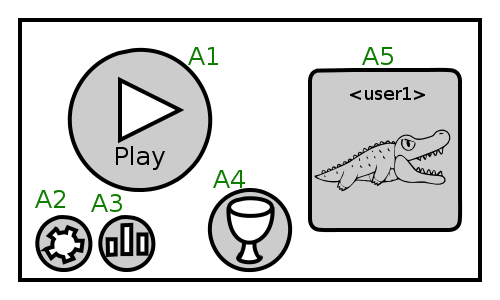
\includegraphics[scale=0.5]{Systemmodelle/images/main_menu.png}
}
\captionof{figure}{Hauptmenü}
\end{center}

Wird beim Neustarten der App als Erstes geöffnet. Wird die App zum Ersten mal verwendet, oder existieren keine Profile, wird zunächst die Profilerstellung (Teil 1) geöffnet.
\begin{requirements}
\req{A1} Öffnet die Levelübersicht.
\req{A2} Öffnet das Einstellungsmenü.
\req{A3} Öffnet die Statistiken. Übernimmt den aktuellen Benutzer als ausgewählten Benutzer in der Statistik.
\req{A4+} Öffnet die Achievements.
\req{A5+} Öffnet die Profilauswahl.
\end{requirements}

\subsubsection{Levelübersicht}

\begin{center}
\setlength\fboxsep{20pt}
\setlength\fboxrule{1pt}
\fbox{
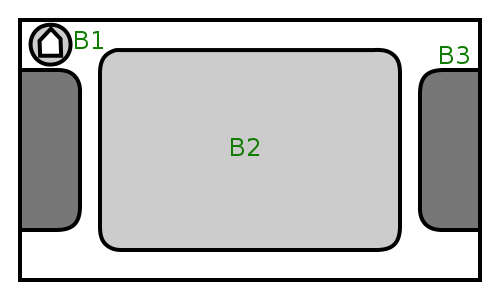
\includegraphics[scale=0.5]{Systemmodelle/images/level_overview.png}
}
\captionof{figure}{Levelübersicht}
\end{center}

\begin{requirements}
\req{B1} Navigiert zurück zum Hauptmenü.
\req{B2} Ein Levelblock. Repräsentiert eine bestimmte Anzahl und/oder Kategorie von elementaren Leveln. Der Sandbox-Modus wird durch einen Levelblock repräsentiert[+]. Öffnet die Leveldetailübersicht.
\req{B3} Der in der Levelanordnung nächste Levelblock. Wird durch eine Swipe-Eingabe zentriert und nimmt so den Platz des aktuellen Levelblocks ein.
\end{requirements}

\subsubsection{Leveldetailübersicht}

\begin{center}
\setlength\fboxsep{20pt}
\setlength\fboxrule{1pt}
\fbox{
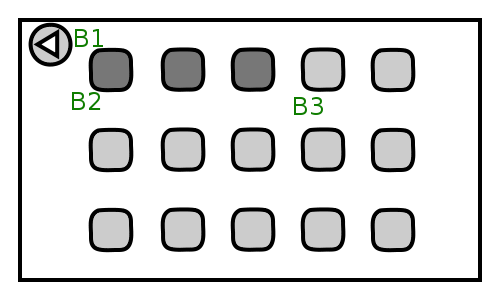
\includegraphics[scale=0.5]{Systemmodelle/images/level_overview_detail.png}
}
\captionof{figure}{Leveldetailübersicht}
\end{center}

\begin{requirements}
\req{C1} Navigiert zurück zur Levelübersicht.
\req{C2} Ein verfügbares Level. Startet das jeweilige Level.
\req{C3} Ein nicht verfügbares Level. Kann durch erfolgreiches Lösen der vorhergehenden Level freigeschaltet werden und wird dann verfügbar.
\end{requirements}

\subsubsection{Level (Platziermodus)}

\begin{center}
\setlength\fboxsep{20pt}
\setlength\fboxrule{1pt}
\fbox{
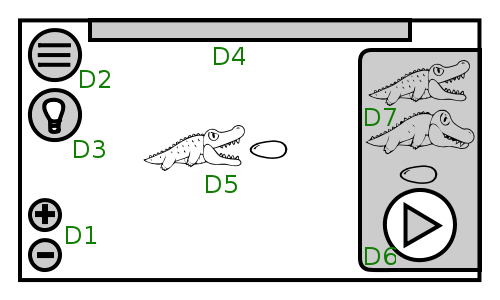
\includegraphics[scale=0.5]{Systemmodelle/images/level.png}
}
\captionof{figure}{Level (Platziermodus)}
\end{center}

\begin{requirements}
\req{D1} Zoom: Vergrößert/verkleinert die Termansicht. Kann im Einstellungsmenü deaktiviert bzw. aktiviert werden.
\req{D2} Öffnet das Spielmenü.
\req{D3+} Öffnet einen Tipp zur Lösung des Levels. Wird erst nach einer gewissen Zeit, in der das Level nicht gelöst werden konnte, aktiviert.
\req{D4} Anwählen oder nach unten Ziehen zeigt die zur Lösung des Levels zu erreichende Konstellation.
\req{D5} Arbeitsfläche. Auf dieser Fläche können zu den bereits vom Level vorgegebenen Alligatoren weitere hinzugefügt werden. Anwählen von platzierten Alligatoren öffnet eine Farbübersicht, aus der eine Farbe für diesen Alligator ausgewählt werden kann.
\req{D6} Startet den Simulationsmodus.
\req{D7} Alligatoren/Eier, die per Drag\&Drop auf der Arbeitsfläche platziert werden können.
\end{requirements}

\subsubsection{Level (Simulationsmodus)}

\begin{center}
\setlength\fboxsep{20pt}
\setlength\fboxrule{1pt}
\fbox{
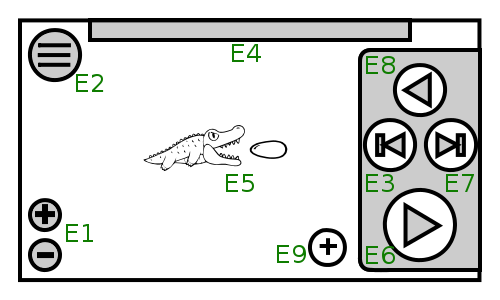
\includegraphics[scale=0.5]{Systemmodelle/images/level_simulation.png}
}
\captionof{figure}{Level (Simulationsmodus)}
\end{center}

\begin{requirements}
\req{E1} Zoom: Vergrößert/verkleinert die Termansicht. Kann im Einstellungsmenü deaktiviert bzw. aktiviert werden.
\req{E2} Öffnet das Spielmenü.
\req{E3+} Setzt, sofern möglich, die Simulation um einen Schritt zurück.
\req{E4} Anwählen oder nach unten Ziehen zeigt die zur Lösung des Levels zu erreichende Konstellation.
\req{E5} Arbeitsfläche. Im Simulationsmodus kann diese nicht mehr verändert werden.
\req{E6} Startet/pausiert den automatischen Simulationsdurchlauf.
\req{E7} Führt einen einzelnen Schritt der Simulaton aus.
\req{E8} Bricht die Simulation ab und kehrt zum Platziermodus zurück.
\req{E9+} Einstellungsmöglichkeit für die Geschwindigkeit der automatischen Simulation. Es stehen zwei Geschwindigkeitsstufen zur Verfügung.
\end{requirements}

\subsubsection{Levelerfolg}

\begin{center}
\setlength\fboxsep{20pt}
\setlength\fboxrule{1pt}
\fbox{
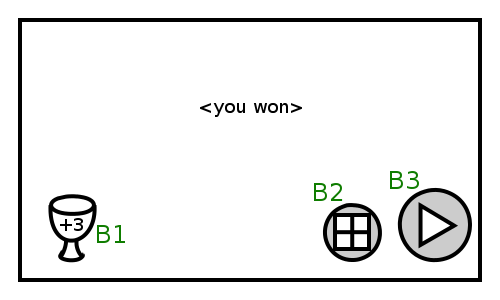
\includegraphics[scale=0.5]{Systemmodelle/images/level_solved.png}
}
\captionof{figure}{Levelerfolg}
\end{center}

Erscheint, sobald im Simulationsmodus ersichtlich ist, dass das Levelziel erfüllt wurde, also, dass die vorgegebene Endkonstellation oder die erforderliche Anzahl an Auswertungsschritten erreicht wurde.
\begin{requirements}
\req{F1+} Stellt die Anzahl der hinzugewonnenen Achievements dar.
\req{F2} Navigiert zur Levelübersicht.
\req{F3} Startet automatisch das nächste Level, sofern möglich.
\req{F4} Startet das aktuelle Level erneut.
\end{requirements}

\subsubsection{Spielmenü}

\begin{center}
\setlength\fboxsep{20pt}
\setlength\fboxrule{1pt}
\fbox{
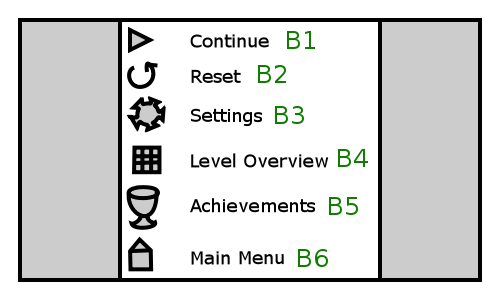
\includegraphics[scale=0.5]{Systemmodelle/images/ingame_menu.png}
}
\captionof{figure}{Spielmenü}
\end{center}

\begin{requirements}
\req{G1} Wechselt zurück zum laufenden Level.
\req{G2} Öffnet das Level im Startzustand. Verwirft den aktuellen Zustand des Levels.
\req{G3} Öffnet das Einstellungsmenü.
\req{G4} Navigiert zurück zur Leveldetailübersicht.
\req{G5+} Öffnet die Achievements.
\req{G6} Navigiert zurück zum Hauptmenü.
\end{requirements}

\subsubsection{Achievements}

\begin{center}
\setlength\fboxsep{20pt}
\setlength\fboxrule{1pt}
\fbox{
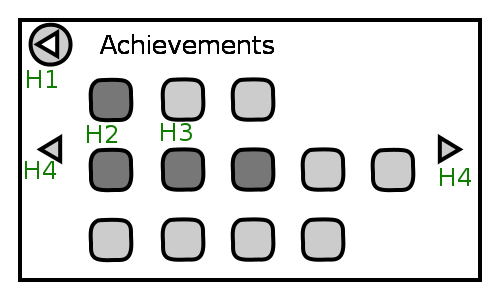
\includegraphics[scale=0.5]{Systemmodelle/images/achievements.png}
}
\captionof{figure}{Achievements}
\end{center}

\begin{requirements}
\req{H1+} Navigiert zurück zum vorigen Navigationpunkt (Spielmenü oder Hauptmenü).
\req{H2+} Erreichtes Achievement. Öffnet die Detailansicht mit Icon und Beschreibung des angewählten Achievements.
\req{H3+} Noch nicht erreichtes Achievement. Ist wahlweise ausgegraut oder unsichtbar. Öffnet, falls nicht unsichtbar, eine Beschreibung, wie das gewählte Achievement zu erreichen ist.
\req{H4+} Navigiert zum vorigen/nächsten Achievementblock.
\end{requirements}

\subsubsection{Achievement-Benachrichtigung}

\begin{center}
\setlength\fboxsep{20pt}
\setlength\fboxrule{1pt}
\fbox{
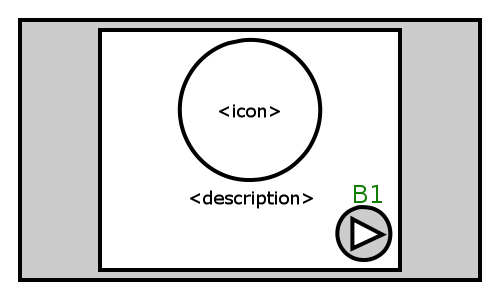
\includegraphics[scale=0.5]{Systemmodelle/images/achievement_notification.png}
}
\captionof{figure}{Achievement-Benachrichtigung}
\end{center}

Alle Achievement-Benachrichtigungen werden nach erfolgreichem Abschluss eines Levels angezeigt.
\begin{requirements}
\req{I1+} Schließt die Benachrichtigung. Wurden weitere Achievements erreicht, erscheint die nächste Benachrichtigung, ansonsten wird mit dem üblichen Levelschema fortgefahren. 
\req{I2+} Icon des Achievements. Öffnet die Achievements.
\end{requirements} 

\subsubsection{Einstellungsmenü}

\begin{center}
\setlength\fboxsep{20pt}
\setlength\fboxrule{1pt}
\fbox{
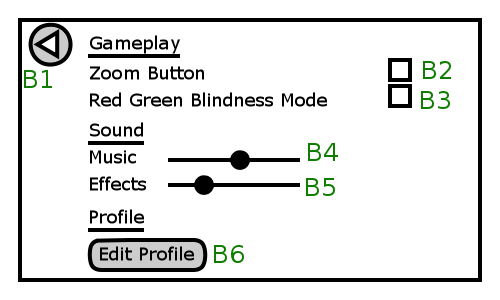
\includegraphics[scale=0.5]{Systemmodelle/images/settings.png}
}
\captionof{figure}{Einstellungsmenü}
\end{center}

\begin{requirements}
\req{J1} Navigiert zurück zum vorigen Navigationpunkt (Spielmenü oder Hauptmenü).
\req{J2} (De-)Aktiviert die buttongesteuerte Zoomfunktion im Level (statt dem üblichen Multitouch-Zoom).
\req{J3+} (De-)Aktiviert den Farbenblindheitsmodus.
\req{J4+} Setzt die Musiklautstärke.
\req{J5+} Setzt die Effektlautstärke.
\req{J6+} Öffnet ein Menü mit den Optionen zum Bearbeiten des Profils (Name ändern/Profilbild ändern/Löschen).
\end{requirements}

\subsubsection{Statistiken}

\begin{center}
\setlength\fboxsep{20pt}
\setlength\fboxrule{1pt}
\fbox{
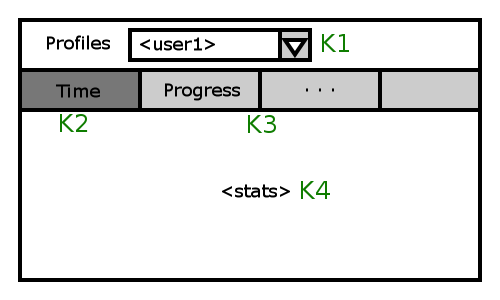
\includegraphics[scale=0.5]{Systemmodelle/images/stats.png}
}
\captionof{figure}{Statistiken}
\end{center}

\begin{requirements}
\req{K1+} Aktuell ausgewählter Benutzer. Beim Öffnen der Statistiken ist der Benutzer gewählt, von dessen Profil aus die Statistiken geöffnet wurden. Öffnet ein Dropdownmenü zur Auswahl eines Benutzers.
\req{K2} Aktuell ausgewählter Tab.
\req{K3} Restliche thematische Tabs. Können durch Touch-Eingabe gewählt oder durch Swipe-Navigation erreicht werden. Tableiste kann je nach Anzahl der Tabs gescrollt werden.
\req{K4} Statistikeinträge. Sind durch Tableiste thematisch gruppiert. Können je nach Anzahl der Einträge gescrollt werden.
\end{requirements}

\subsubsection{Profilauswahl}

\begin{center}
\setlength\fboxsep{20pt}
\setlength\fboxrule{1pt}
\fbox{
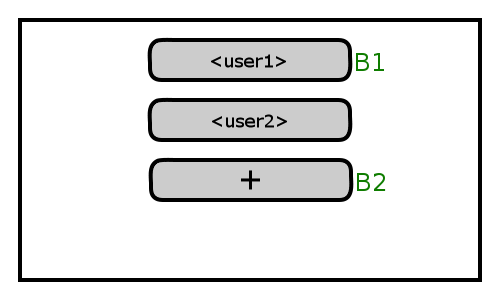
\includegraphics[scale=0.5]{Systemmodelle/images/change_user.png}
}
\captionof{figure}{Profilauswahl}
\end{center}

\begin{requirements}
\req{L1+} Selektiert das gewählte Profil und öffnet dessen Hauptmenü.
\req{L2+} Öffnet den Profilerstellungsdialog.
\end{requirements}

\subsubsection{Profilerstellung(Teil 1)}

\begin{center}
\setlength\fboxsep{20pt}
\setlength\fboxrule{1pt}
\fbox{
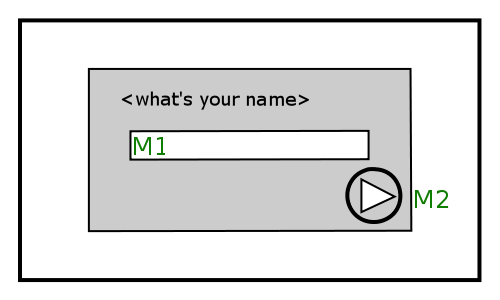
\includegraphics[scale=0.5]{Systemmodelle/images/profile_creator_1.png}
}
\captionof{figure}{Profilerstellung (Teil 1)}
\end{center}

Wird bei erstmaliger Benutzung der App als Erstes geöffnet.
\begin{requirements}
\req{M1} Texteingabefeld für den Benutzernamen. Öffnet die Tastatur.
\req{M2+} Bestätigt den eingegebenen Namen und fährt mit Profilerstellung (Teil 2) fort. Falls der eingegebene Name ungültig (z.B. leer) ist oder schon ein Profil mit diesem Benutzernamen existiert, wird eine entsprechende Meldung und eine Möglichkeit zur Änderung der Eingabe gegeben.
\end{requirements}

\subsubsection{Profilerstellung(Teil 2)}

\begin{center}
\setlength\fboxsep{20pt}
\setlength\fboxrule{1pt}
\fbox{
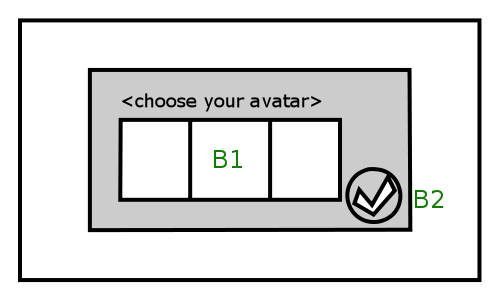
\includegraphics[scale=0.5]{Systemmodelle/images/profile_creator_2.png}
}
\captionof{figure}{Profilerstellung (Teil 2)}
\end{center}

\begin{requirements}
\req{N1+} Wahlmöglichkeiten für das Profilbild. Selektiert und markiert das gewählte Bild. Wird eventuell durch einen umfangreicheren Dialog ersetzt.
\req{N2+} Bestätigt das ausgewählte Bild, erstellt ein Profil und öffnet dessen Hauptmenü.
\end{requirements}

